\documentclass{article}
\usepackage{graphicx}
\usepackage{amsmath,amsthm,amssymb}
\usepackage[font=small,labelfont=bf]{caption}
\usepackage{tikz}
\usepackage{pgfplots}
\pgfplotsset{compat=1.18}
\usetikzlibrary{calc, angles, quotes, shapes.geometric, decorations.pathreplacing}
\usepackage{tkz-euclide}
\usepackage[inline]{asymptote}
\usepackage{float}
\usepackage[margin=1in]{geometry}
\usepackage{gensymb}
\usepackage[normalem]{ulem}
\usepackage{hyperref}
\hypersetup{
    colorlinks=true,
    linkcolor=blue,
    filecolor=magenta,      
    urlcolor=cyan,
    pdftitle={Overleaf Example},
    pdfpagemode=FullScreen,
    }
\usepackage{fancyhdr}
\pagestyle{fancy}
\fancyhead[R]{Enoch Yu}
\pagenumbering{gobble}
\usepackage{enumitem}
\newtheorem{theorem}{Theorem}[section]
\newtheorem{lemma}[theorem]{Lemma}
\newtheorem*{lemma*}{Lemma}
\newtheorem{sublemma}{Lemma}[section]
\newtheorem{proposition}{Proposition}
\newtheorem{corollary}{Corollary}[theorem]
\newtheorem{example}{Example}[section]
\newtheorem*{example*}{Example}
\newenvironment{solution}{\begin{trivlist}\item[]{\bf Solution}}{\qed \end{trivlist}}
\newcommand{\verteq}{\rotatebox{90}{$\;\;=\;\;$}}
\newcommand*\circled[1]{\tikz[baseline=(char.base)]{
            \node[shape=circle,draw,inner sep=1pt] (char) {#1};}}
\newcommand{\triangled}[1]{\tikz[baseline=(char.base)]{
            \node[shape=regular polygon, regular polygon sides=3, draw, inner sep=0.2pt] (char) {#1};}}

\title{Problem Set 23}
\author{Enoch Yu}
\date{June 2025}

\begin{document}

\section*{Problem}
How many solutions are there to the equation $\log_3 x = 3 \sin(3 \pi x)$?
\begin{solution}
\\\\
\textbf{Key Word} Graphing
\begin{center}
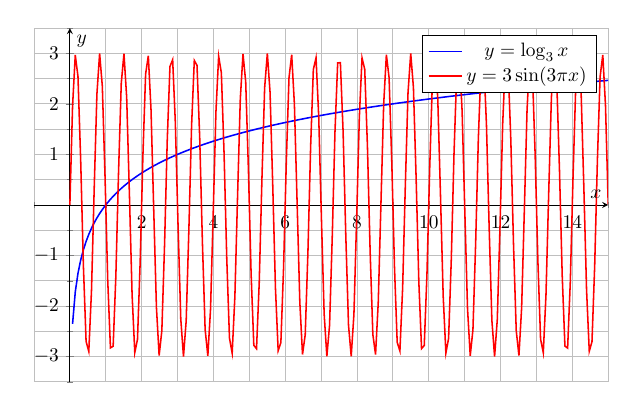
\begin{tikzpicture}[scale=0.7]
  \begin{axis}[
    axis lines = middle,
    xlabel = {$x$},
    ylabel = {$y$},
    xmin=-1, xmax=15,
    ymin=-3.5, ymax=3.5,
    width=12cm,
    height=8cm,
    legend style={at={(0.98,0.98)},anchor=north east},
    grid=both,
    minor tick num=1,
    ]

    \addplot[blue, thick, samples=200, domain=0:15] {ln(x)/ln(3)};
    \addlegendentry{$y = \log_3 x$}

    \addplot[red, thick, samples=200, domain=0:15] {3*sin(deg(3*pi*x))};
    \addlegendentry{$y = 3 \sin(3\pi x)$}
  \end{axis}
\end{tikzpicture}
\end{center}
Looking at the graph, it is evident that two intersection occurs for each period except for the first period, where each has one intersection. Moreover, there exists $40$ periods since $\frac{27}{\frac{2}{3}} = \frac{81}{2}$.
\[
\therefore 1 + 39 \cdot 2 + 2= \boxed{81}
\]
\end{solution}

\newpage
\section*{Problem}
In $\triangle{ABC}$, $AC = 6$ and $BC = 17$. If $\tan\frac{A}{2}\tan\frac{C}{2} = \frac{2}{3}$, find $AB$.C
\begin{solution}
\\\\
\textbf{Key Word} Law of Sines, Law of Cosines, Trigonometric Identities
\\\\
First and foremost the situation could be drawn.
\begin{center}
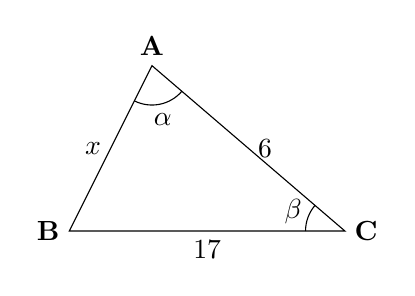
\begin{tikzpicture}[scale=0.7]
  \coordinate (A) at (1.5,3);
  \coordinate (B) at (0,0);
  \coordinate (C) at (5,0);
  \draw (A) -- (B) -- (C) -- cycle;
  
  \node[left] at (B) {\textbf{B}};
  \node[right] at (C) {\textbf{C}};
  \node[above] at (A) {\textbf{A}};
  
  \node[left] at ($(A)!0.5!(B)$) {$x$};
  \node[right] at ($(A)!0.5!(C)$) {$6$};
  \node[below] at ($(B)!0.5!(C)$) {$17$};
  
  \draw pic["$\alpha$", draw=black, angle radius=0.5cm, angle eccentricity=1.4] {angle=B--A--C};
  \draw pic["$\beta$", draw=black, angle radius=0.5cm, angle eccentricity=1.4] {angle=A--C--B};
\end{tikzpicture}
\end{center}
Using the law of sines, the following equation could be driven.
\begin{align*} 
    \frac{\sin\alpha}{17} &= \frac{\sin\beta}{x} \\
    \frac{\sin\beta}{\sin\alpha} &= \frac{x}{17}
\end{align*}
Moreover, using trigonometric identities, the following relationships could be found.
\begin{align*}
    \tan\frac{\theta}{2} = \frac{\sin\frac{\theta}{2}}{\cos\frac{\theta}{2}}
    &= \frac{\sqrt{\frac{1 - \cos\theta}{2}}}{\sqrt{\frac{1 + \cos\theta}{2}}} \\[0.5em]
    &= \frac{\sqrt{1 - \cos\theta}}{\sqrt{1 + \cos\theta}} \\[0.5em]
    &= \frac{\sqrt{1 - \cos\theta}}{\sqrt{1 + \cos\theta}} \cdot \frac{\sqrt{1 + \cos\theta}}{\sqrt{1 + \cos\theta}} = \frac{\sin\theta}{1 + \cos\theta} \\[0.5em]
    &= \frac{\sqrt{1 - \cos\theta}}{\sqrt{1 + \cos\theta}} \cdot \frac{\sqrt{1 - \cos\theta}}{\sqrt{1 - \cos\theta}} = \frac{1 - \cos\theta}{\sin\theta}
\end{align*}
Therefore, the two relationships could be applied alternately.
\begin{align*}
    \frac{1 - \cos A}{\sin A} \cdot \frac{\sin C}{1 + \cos C} = \frac{1 - \cos\alpha}{\sin\alpha} \cdot \frac{\sin\beta}{1 + \cos\beta} &= \frac{2}{3} \\
    \frac{\sin\beta}{\sin\alpha} \cdot \frac{1 - \cos\alpha}{1 + \cos\beta} = \frac{x}{17} \cdot \frac{1 - \cos\alpha}{1 + \cos\beta} &= \frac{2}{3} \\
    \frac{x}{17} \cdot \frac{1 - \frac{x^2 + 6^2 - 17^2}{2 \cdot 6 \cdot x}}{1 - \frac{17^2 + 6^2 - x^2}{2 \cdot 17 \cdot 6}} = \frac{x}{17} \cdot \frac{17}{x} \cdot \left( \frac{2 \cdot 6 \cdot x - x^2 - 6^2 + 17^2}{2 \cdot 17 \cdot 6 - 17^2 - 6^2 + x^2} \right) &= \frac{2}{3} \\
    \frac{-(x - 6)^2 + 17^2}{-(17 - 6)^2 + x^2} = \frac{(17 + x - 6)((17 - x + 6)}{(x + 11)(x - 11)} &= \frac{2}{3} \\
    \frac{23 - x}{x - 11} &= \frac{2}{3} \\
    \therefore x &= \boxed{\frac{91}{5}}
\end{align*}
\end{solution}


\end{document}
